\chapter{De architectuur van de blockchain technologie}
Dit hoofdstuk gaat verder in op de basisarchitectuur van de blockchain. Zodat tijdens het ontwikkelen van het Proof of Concept, de basisbegrippen van de technologie correct worden begrepen.

\section{Blok (block)}
Zoals al eerder was aangegeven is de blockchain een gedistribueerd grootboeksysteem. Gegevens worden permanent opgeslagen in het netwerk via bestanden die blokken worden genoemd. Een blok is een document waarin recente transacties van een bepaald moment zijn vastgelegd. Het heeft daarom de naam blockchain, omdat het een reeks van blokken zijn die steeds maar naar de vorige verwijst. Een nieuwe blockchain database begint daarom met een zogenaamd genesis blok \cite{blochchainTechSymmbioticDev}.\par
					
Een blok in het geval van de Bitcoin bestaat uit een header en een body \cite{blockchainIssuesAndChallenges}. De header bestaat uit drie stukken metagegevens. De eerste is een verwijzing naar een vorige blockhash (Merkle-hash \footnote{https://en.wikipedia.org/wiki/Merkle\_tree}). Hierdoor verbindt het blok met de vorige uit de blockchain. De tweede set van metagegevens is moeilijkheidsgraad, tijdstempel en nonce\footnote{https://en.wikipedia.org/wiki/Cryptographic\_nonce}. Het laatste stuk metadata is de Merkle-tree root, een datastructuur die wordt gebruikt om alle transacties in het blok efficiënt samen te vatten \cite{masteringBitcoin}.

\begin{figure}[h]
    \begin{center}
        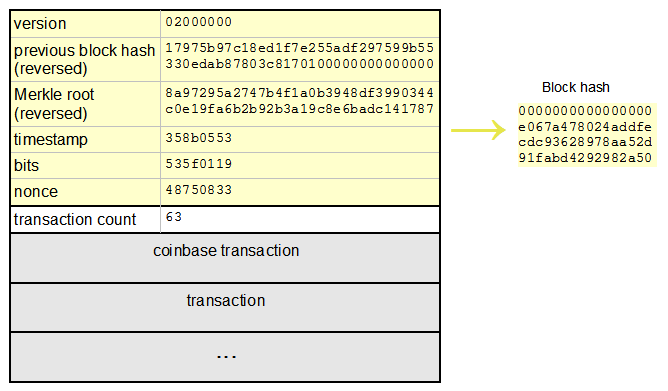
\includegraphics[width=\paperwidth-335pt]{images/block}
        \caption{Illustreert de structuur van een block in de bitcoin blockchain.\\Bron: http://www.righto.com/2014/09/mining-bitcoin-with-pencil-and-paper.html}
        \label{fig:blockchain?}
    \end{center}
\end{figure}
\newpage

\section{Gedecentraliseerd netwerk}\label{cap:decentralisedNetwork}
Interacties tussen gebruikers op de blockchain gebeuren hoofdzakelijk gedecentraliseerd. Dit betekent dat iedere gebruiker een punt vertegenwoordigt van het netwerk. Iedere gebruiker heeft dezelfde blockchain software geïnstalleerd en is direct verbonden met een aantal andere gebruikers van het netwerk. Wanneer een gebruiker een transactie uitvoert met een andere gebruiker dan ontvangen de andere gebruikers deze informatie ook. Deze gebruikers valideren ze dan eerst en sturen het vervolgens door als het klopt \cite{challengesOppertunities}.\par

Het voordeel van een gedecentraliseerd netwerk, is dat geen centraal punt is die kan falen of de beheerdersrol kan hebben. Hierdoor wordt de menselijke factor geminimaliseerd en het vertrouwen verschuift van centrale organisatie naar vertrouwen in de open source code waaraan meerdere auteurs aan werken\cite{stateNecessary}.
\newpage

\section{Consensus (overeenstemming) algoritmes}\label{cap:consensus}
Om de werking van de blockchain te begrijpen en te vertrouwen, moet het begrip van Consensus oftewel overeenstemming algoritmes  duidelijk zijn. Deze algoritmes worden gebruikt wanneer een (nieuw) blok aan informatie geverifieerd wordt. Het zorgt voor één historie van transacties waar de geschiedenis geen ongeldige of tegenstrijdige transacties bevat.\par

Dit is allemaal nodig omdat de blockchain draait in een zelf gereguleerde, wantrouwende omgeving waar het nodig is om meningsverschillen over transacties binnen het netwerk op een lijn te krijgen. Het zorgt ervoor dat er niet één account is die meer uitgeeft dan dat het heeft, of waar hij of zij twee keer iets overmaakt, dit heet double-spending. De bekende consensus algoritmes zijn proof of work en proof of stake:\par

\begin{enumerate}
	\item Proof of Work (PoW)\\
	Het PoW consensus algoritme is het meest voorkomende algoritme in blockchain. Het werd geïntroduceerd door de Bitcoin en gaat ervan uit dat alle peers met rekenkracht mee stemmen door PoW-instanties, cryptografische puzzels op te lossen en hiermee het recht hebben om de volgende blok aan te maken in het netwerk. Zo maakt de Bitcoin gebruik van een hash-gebaseerde PoW, wat inhoudt dat de peers een nonce-waarde\footnote{https://en.wikipedia.org/wiki/Cryptographic\_nonce} proberen te vinden. Wanneer een dergelijke nonce wordt gevonden, maakt de miner het blok aan en stuurt hij het door naar zijn peers. Deze peers ontvangen dit dan en verifiëren of het klopt aan de hand van het vorige blok  \cite{securityPOW}.
	\item Proof-of-Stake (PoS)\\
Op het moment moet Proof-of-Stake zich nog bewijzen in de crypto valuta gemeenschap. Het is ontwikkeld om bestaande inefficiënte consensus algoritmes zoals PoW te vervangen. Het algemeen begrip van PoS is dat een deelnemer van de blockchain, pas het stemrecht heeft op een nieuwe blok in de blockchain als de peer zich voldoende heeft ingezet in het netwerk. In het geval van PeerCoin\footnote{https://peercoin.net/} worden nieuwe blokken gegeneerd door het netwerk op basis van niet gespendeerde valuta en hoe oud deze is \cite{posProtocol}.\par

Met deze methode wordt aangenomen dat oude deelnemers van het netwerk minder snel het netwerk zullen aanvallen \cite{blockchainIssuesAndChallenges}. Dit lost op het gebied van energiebesparing de problemen van PoW op, waar gebruikers miners aanzetten om valuta te ontvangen. Bij PoS wordt de valuta die niet beweegt steeds meer waard.
\end{enumerate}
\newpage

\section{Smart contract}
Het idee achter smart contracts is een "geautomatiseerd transactie protocol dat de voorwaarden van een contract uitvoert" \cite{smartContracts} en werd voor het eerst bedacht door cryptograaf Nick Szabo. Dit idee is door de opkomst van de blockchain populair geworden. Dit komt doordat de blockchain gedecentraliseerd is en daardoor de tussenpersonen bij een gecentraliseerde smart contracts applicatie eruit haalt. Smart contracts is, in de context van blockchain, gewoon software die op een blockchain wordt gepubliceerd en die transacties kan ontvangen of uitvoeren. Iedere transactie heeft een adres en kan worden gevolgd.\par